\chapter{Preliminary report}

\subsection*{Introduction}

Quantum computing has the potential to transcend the information technology as we know it. Small scale quantum systems are already possible today and the goal is to scale up these quantum architectures to build practical quantum devices. One approach to do this is to by networking many simple processor cells together through quantum links, avoiding the necessity to build a single complex structure. Processor cells that are located physically close to each other are connected by "short" links and lie in a patch. Patches that are located physically far from each other can in turn be connected by "long" links, such as remote optical connections. The total state of system, which contains the stored information, is shared across these patches, such that it can be accessed in either one of these patches. \\

This is somewhat analogous to the idea of a shared database. Many online services that we use today rely on servers that host the data that we want to view, store or edit. This data is often not stored on a single server, but copied to many others, in a shared database. In case one of these servers goes offline due to file corruption or an electricity outrage, the data is not lost, and can still be accessed on another server in the cluster.\\

In our Quantum network, information cannot be copied across different processor cells due to the no cloning theorem. In stead, it is shared across cells through entanglement. A cell can also go "offline", when a qubit or multiple qubits are lost from the system due to some interaction with the environment. This process is called decoherence, also described with \emph{loss} or \emph{erasure}. Luckily, if the losses are not too much, these cells can be restored through quantum error correction (QEC) such that the quantum state or encoded information can still be extracted from the system. \\

\subsection*{Quantum errors}
Errors that can occur during Quantum computation can generally be classified as 1) noise, in which there is an error are within the computational basis, or as 2) a loss, in which the qubit is
taken out of the computational basis. Losses are both detectable and locatable, which means that a higher rate of loss ($p_{loss}$) can be tolerated than noise or computational errors ($p_{com}$). The process of finding and correcting these errors is called decoding. \\

Kitaev's surfaces codes are defined by a set of stabilizers which act on a set of physical qubits that lie on the edges of a square lattice \cite{kitaev}. The stabilizers commute, and are generated by plaquettes (group of $Z$ operators), or by stars (group of $X$ operators). Logical operates corresponds to a set of stabilizer operators along a homologically nontrivial cycle. Any homologically equivalent set of operators can be used to measure the physical qubit operator. Therefore, in the case of a qubit loss, another set of operators can be used, if there is no \emph{percolated} region of losses that span the entire lattice. \\

To decode for computational errors, one measures the stabilizer generators, which returns eigenvalue -1 on the edges of the error chains or syndromes, and can be corrected by finding a nontrivial closing chain, which either equals a stabilizer measurement that corrects the error, or a logical operator which equals a logical error. This problem is equivalent to the two dimensional random-bond Ising model (RBIM), where the shortest path needs to be found between matching pairs. The closing chain is found using the Edmonds' minimum weight perfect matching (MWPM) algorithm. This algorithm scales quadratic in time as the lattice size increases \cite{stace2009}. More recently, an almost-linear decoding approach has been described by Delfosse et al. \cite{nickerson2017}. \\

There are also multiple methods to decode for losses on the surface code. Stace et. al \cite{stace2009,stace2010} describes the method of so-called superplaquettes and superstars, in which the lost qubit is accounted for by combining neighboring stabilizers. The resulting lattice can be than decoded using the same MWPM algorithm. Delfosse et al \cite{delfosse2017} describes a linear-time maximum likelihood method to decode for losses. Here, the errors are found in a \emph{peeling} algorithm that iteratively peels branches away from a tree of possible error chains until the lost qubits remain.

\subsection*{Patch loss}
In terms of the surface code, a patch is a set of neighboring qubit cells on the lattice that lie physically close to each other. The entire lattice is built by connecting multiple patches. It is possible that cells within the same patch suffer the same decoherence, due to their physical vicinity, such that entire patches may be lost. The Quantum links that connect these patches, in turn, may suffer a larger amount of noise due to the distance it must cross. \\

These patch losses may be investigated using the decoding algorithms described above. There are two main question to be answered here. The first one involves the size of the patches. What are tolerable sizes of patches such that in the event of a patch loss, the encoded Quantum information can still be extracted from the system? The second question concerns the Quantum links between these patches. What effects does the patch model on the surface have on the tolerable noise thresholds, especially on the thresholds of the Quantum links that connect different patches?

\subsection*{Project}
This project will focus on the two problems of the patch model described in the previous section. We will use simulations to calculate for the thresholds on patch sizes and noise. Most probably, we will try to build this simulation on top of the fault-tolerance simulations by N. Nickerson \cite{naomi}, whose thesis will also be used as our foundation on quantum error correction. Furthermore, the introduction on topological codes will be provided by the lecture notes of D. Browne \cite{browne}. We we use the knowledge acquired in the courses Advanced Quantum Mechanics (AP3051G), Computational Physics (AP3082D), as well as the EDX courses The Building Blocks of a Quantum Computer (DelftX - QTM2x, QTM3x) and Quantum Cryptography (CaltechDelftX - QuCryptox), which are similar to the TU Delft courses AP3421 and CS4090. \\

The project will be done under supervision of David Elkouss, who leads the Elkouss group, which is part of the Roadmap Quantum Internet and Networked Computing at QuTech. Weekly meetings are planned for discussions and evaluations. A presentation for the group will be held after a month. Furthermore, we also expect to be working closely together with Sebiastian de Bone, who is a Phd student at the Elkouss Group.\\

\noindent
The project can be divided into 5 successive objectives:
\begin{enumerate}\label{test}
  \item Theory and prediction of model with patch-loss of the surface code.
  \item Calculation of threshold on patch sizes.
  \item Definitions of noise between patches.
  \item Combine patch-loss and noise between patches.
  \item Improve decoder.
\end{enumerate}
The preparation for the master thesis ends on April 12, 2019. From here, the first 3 months of the project, until July 2019, we expect to be working on objective 1, expanding our theoretical knowledge of the Quantum erasure code and formulating definitions of the patch model. Ideally, we will also have some simulations results for objective 2 by the end of July. We will take a short break in August, whereafter we will continue on objectives 3 and 4. Objective 5, improving the decoder, is an optional objective. The mechanism of the decoders are so complicated, that an improvement may be a project on its own. However, due to my particular interest in these decoders, I will be alert on trying to find a point of improvement if possible. The timeline of this project will look as such.
\begin{figure}[htpb]
  \centering
  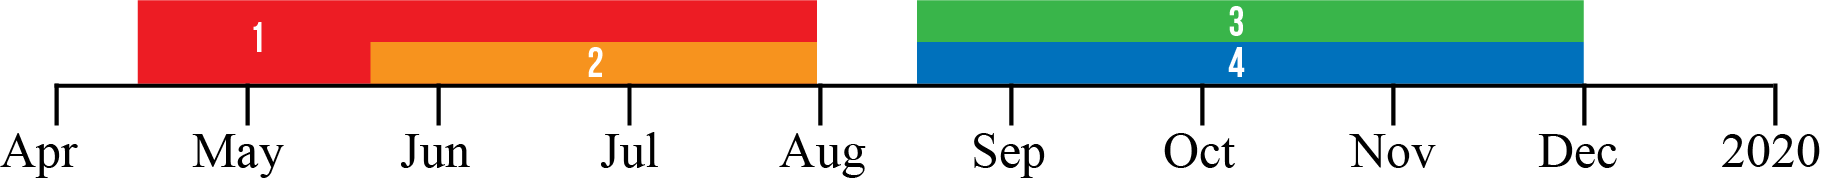
\includegraphics[width=\linewidth]{fig/Timeline.png}
\end{figure}

If the simulation of the patch sizes (2) will be so complicated such that after it cannot be completed before the end of July, we will drop objectives 3 and 4 and focus on the first two objectives. The deadline for the thesis is set to the end of November, such that a defense may be held in December.


%In the case that $p_{com} = 0$, the threshold for logical qubit recovery is $p_{loss} < 0.5$, which is equivalent to the \emph{bond percolation threshold}. In the case that $p_{loss} = 0$, computational errors can be found by measuring the stabilizer generators, which returns eigenvalue -1 on the edges of the error chains or syndromes, and can be corrected by finding a nontrivial closing chain, which either equals a stabilizer measurement that corrects the error, or a logical operator which equals a logical error. This problem is equivalent to the two dimensional random-bond Ising model (RBIM), where the shortest path needs to be found between matching pairs. The closing chain is found using the Edmonds' minimum weight perfect matching (MWPM) algorithm. In this case, the threshold is $p_{com} < 0.104$, for which a larger lattice size will decrease the chance of a logical error. These two thresholds corresponds to two end points of a boundary of correctability: $(p_{loss}, p_{comp}) = (0.5,0)$ and $(0,0.104)$.\\

%\subsubsection*{Superstabilizer decoder\cite{stace2009,stace2010}}
%To correct for losses on the surface code, new stabilizer generators are formed by connecting neighboring plaquettes or stars, which are connected to the same lost qubit, forming so-called superplaquettes and superstars respectively. These superstabilizers may share multiple qubits, and a nontrivial error chain arises of there are an odd number of (computational) errors in these shared qubits. This can be avoided by degrading the edges (shared qubits) between the superstabilizers to a single superedge whose error rates depend on the number of physical qubits shared, accounting for this degeneracy. For the sake of computation it is easier to stay on a square lattice. Take each stabilizer as a node and each shared qubit as an edge. The superstabilizer approach can be achieved by setting the weight of the edge of a lost qubit to 0, and the weight of shared edges between superstabilizers to the weight of the superedge. \\

%Using the superstabilizer approach, Edmonds' MWPM algorithm can be applied with altered edge weights. Simulations using the superstabilizers scheme with varying $p_{loss}$ show that the computational error threshold $p_{comp}^{thr}$ stay within the boundary of correctability, following the universal scaling law. At the limit of small $p_{loss}$, superstabilizer mostly consist of only 6 qubits, and increasing $p_{loss}$ only contributes to the number of superstabilizers, resulting in a linear relationship of threshold $p_{comp}^{thr}$ with $p_{loss}$.   As $p_{loss}$ increases further, larger superstabilizers containing more qubits appear, which have an increased chance of syndrome error. At $p_{loss} > 0.425$, the universal scaling law breaks down due to the size of the superstabilizers, as finite lattice effects dominate.\\

%One must also take into account that some error matchings may have a higher path degeneracy than others, indicating that the former is more likely. Therefore, the weights of the edges must additionally account for this degeneracy. However, due to this notion it possible that the algorithm may favor a matching that is not necessarily the shortest path. To balance these factors an additional factor $\tau$ is introduced that specifies the importance of path degeneracy. An optimal value for $\tau$ is found for which the computational error threshold is increased to $p_{comp}^{thr} = 0.1065$. Various implementations of Edmonds' MWPM algorithms are tested not to account for this degeneracy, and therefore a higher threshold may be possible with a computationally efficient algorithms that takes this into account.

%\subsubsection*{Maximum likelihood decoder\cite{delfosse2017}}
%Another way to look at erasure, is that the lost qubit is replaced by a maximally mixed state, which can also be interpreted as a qubit suffering a Pauli error $I,X,Y,Z$ chosen at random. Just as before, the decoding is done by measuring the plaquettes and stars, except now there is the additional knowledge of the erasure pattern, in which the errors must occur.\\

%For a set of errors $\sigma$ in the erasure pattern $\varepsilon$, either $X$ or $Z$ errors ($Y$ is a combination of the two), the algorithm is to make a spanning forest $F_{\varepsilon}$ inside of $\varepsilon$, a maximal subset of edges of $\varepsilon$ that contains no cycles. From this tree, boundary edges called leafs are iteratively stripped from $F_{\varepsilon}$. If the single connected vertex of the leave is in $\sigma$, the leaf or edge is added to the correction chain, and the other vertex is flipped in $\sigma$. What remains after the stripping $F_{\varepsilon}$ is the correction chain. On surface codes with boundaries, additional constrains are applied to the method of how the spanning forest is grown. \\

%\subsubsection*{Comparison}
%The benefit of the maximum likelihood decoder is that it scales linear with the size of the surface code. The spanning forest can be grown in linear-time, and the stripping process also only passes each leaf once, ensuring linear complexity. The superstabilizer decoder applies Edmonds' algorithm, which scales quadratic in time, but does however solve for erasure and computation errors simultaneously, whereas the maximum likelihood decoder only solves for erasure errors. Therefore, the optimal decoder probably depends on the size of the system.
